\documentclass[9pt,conference]{IEEEtran}
\usepackage[utf8]{inputenc}
\usepackage[brazil]{babel}

% Diversos
\usepackage{csquotes}
\usepackage{graphicx}
\usepackage{verbatim}
\usepackage{hyperref}
\usepackage{smartdiagram}

% Título
\title{Utilizando Redes Convolucionais de Grafos Espaço-Temporais para o Reconhecimento da Línguas de Sinais}
%\author{Cleison Correia de Amorim}
\date{Outubro 2018}

\author{
    \IEEEauthorblockN{Cleison Correia de Amorim}
    \IEEEauthorblockA{Centro de Informática\\
    Universidade Federal de Pernambuco\\
    Email: cca5@cin.ufpe.br}
}

% Comandos
% 'image': definição de imagem
\newcommand{\image}[4][\linewidth] {
    \begin{figure}[ht]
    \centering
    \includegraphics[width=#1]{#3}
    \caption{#4}
    \label{#2}
    \end{figure}
}

% 'refimage': referências de imagens
\newcommand{\refimage}[1] {figura \ref{#1}}

% 'refsection': referências de seções
\newcommand{\refsect}[1] {seção "\nameref{#1}"}

\begin{document}
\maketitle
\begin{abstract}
Este trabalho propõe a aplicação de um modelo profundo na transcrição das características fonológicas da língua de sinais para o modelo de descrição computacional CORE-SL. Para isso, será utilizado o modelo de Redes Convolucionais de Grafos Espaço-Temporais, que baseia-se na representação do esqueleto humano na forma de grafos, e no aprendizado automático dos seus padrões de movimentos no espaço e no tempo por meio deles.
\end{abstract}

%\begin{IEEEkeywords}
%Broad band networks, quality of service, WDM.
%\end{IEEEkeywords}


\section{Introdução} %%%%%%%%%%%%%%%%%%%%%%%%%%%%%%%%%%%%%%%%%%%
\label{sec:introducao}
Existe um grande número de estudos que propõem-se a realizar a tradução de diferentes línguas de sinais para a língua falada correspondente. Entretanto, muito desses estudos são limitados frente ao contexto cotidiano do Surdo por desconsiderarem aspectos relevantes da fonologia da língua como os movimentos, expressões não-manuais, locação e orientação das mãos do interlocutor \cite{quadros-2004}. É comum também que tais estudos restrinjam seu campo de atuação ao âmbito da datilologia\footnote{
    Datilologia – também conhecida como alfabeto digital ou alfabeto manual, consiste na soletração de palavras pelos Surdos. É geralmente utilizada para introduzir uma palavra que ainda não possui um sinal equivalente \cite{quadros-2004}\cite{pereira-choi-2011}.
}, que na prática é aplicada apenas em contexto restritos da comunicação desses indivíduos.

Em \cite{antunes-hcisl-2011}, os autores apresentam outros fatores que justificam a limitação em trazer muitos desses estudos para a realidade do Surdo: 
\begin{enumerate}
    \item O uso de equipamentos como luvas, acelerômetros e outros sensores que são de difícil acesso; 
    \item A adoção de métodos e tecnologias que não empatizam com a realidade surdo, restringindo sua movimentação ou deixando de considerar aspectos importantes, como as expressões faciais;
    \item O uso de métodos que mapeiam sinais diretamente para palavras, e que tornam-se facilmente obsoletos mediante a introdução de novos sinais ou quando confrontados com variações linguísticas como gírias e regionalismos; 
    \item A utilização de imagens estáticas para o treinamento de modelos, que desconsideram a dinâmica da língua.
\end{enumerate}

Diante dessas limitações, foi introduzido em \cite{antunes-hcisl-2011} a proposta de uma arquitetura capaz de considerar os aspectos fonológicos da língua e de viabilizar a interação homem-máquina por meio dos sinais, a qual foi denominada HCI-SL. A \refimage{fig:hcisl} apresenta essa arquitetura, onde uma API interna compreendendo tecnologias de visão computacional e processamento de linguagem natural proveem uma interface padrão para ferramentas e serviços externos como dicionários, tradutores e aplicações de finalidades diversas.

\image
	[5cm]
    {fig:hcisl}
    {images/hcisl}
    {Arquitetura HCI-SL apresentada por \cite{antunes-hcisl-2011}.}

Para a arquitetura acima funcionar, foi necessário primeiro definir o CORE-SL, que consiste num modelo computacional para descrição dos sinais e suas características fonológicas. Ele estabelece um padrão de representação a ser adotado pelas peças que compõem a arquitetura HCI-SL e pelas aplicações e serviços desenvolvidos a partir dela.

De acordo com os autores, o CORE-SL:

\begin{quote}
[...] agrega flexibilidade e um nível de detalhamento capazes de proporcionar alternativas para um tratamento computacional robusto e para auxiliar às diferentes necessidades de aplicação. Este modelo atuará como um dos pilares de sustentação na construção de artefatos tecnológicos que considerem as necessidades deste perfil de usuário e tornem a comunicação usuário-sistema natural para ele. \cite{antunes-2011}
\end{quote}

 A \refimage{fig:coresl-interfaces} ilustra as interações do CORE-SL com um conjunto de serviços idealizados ou em desenvolvimento por pesquisadores da Universidade Federal do Paraná - UFPR. Nela, o modelo exerce um papel central para a comunicação das peças envolvidas.

\image
    {fig:coresl-interfaces}
    {images/coresl_interfaces}
    {CORE-SL como peça chave para a comunicação entre serviços \cite{garcia-2013}.}

A \refimage{fig:coresl-sinalarvore} mostra um exemplo de descrição do sinal árvore através do modelo CORE-SL.

\image
    {fig:coresl-sinalarvore}
    {images/sinal_arvore}
    {Representação do sinal árvore escrito segundo o CORE-SL.}
    

\section{Redes Convolucionais de Grafos Espaço-Temporais} %%%%%%%%%%%%%%%%%%%%%%%%%%%%%%%%%%%%%%%%%%%

Para viabilizar a transcrição dos sinais articulados para um modelo de descrição como o CORE-SL, neste trabalho será utilizado o modelo \textit{Spatial-Temporal Graph Convolutional Networks - ST-GCN}\footnote{
    O código fonte do modelo ST-GCN é disponibilizado publicamente pelos autores no endereço \url{https://github.com/yysijie/st-gcn}.
} (ou Redes Neurais de Grafos Espaço-Temporais) proposto em \cite{st-gcn-2018}. Sua escolha deve-se ao fato dele ser centrado na dinâmica do esqueleto humano e ser capaz de lidar com seu movimento sob duas perspectivas distintas e complementares entre si. Esses aspectos tornam a abordagem do ST-GCN extremamente relevante ao contexto da língua de sinais apresentado.

Segundo os autores:
\begin{quote}
A dinâmica dos esqueletos humanos transmite informações significativas para o reconhecimento de sua ação. Abordagens convencionais para modelagem de esqueletos geralmente dependem de partes feitas à mão ou de regras transversais, resultando assim em poder expressivo limitado e dificuldades de generalização. [...] o ST-GCN vai além das limitações dos métodos anteriores, aprendendo automaticamente os padrões espaciais e temporais a partir dos dados. Essa formulação não apenas leva a um maior poder expressivo, mas também a uma capacidade de generalização mais forte \cite{st-gcn-2018}.
\end{quote}

O modelo é formulado com base numa sequência de grafos de esqueletos extraídos de uma sequência de frames de vídeos, onde cada nó corresponde a uma junta do corpo humano, conforme \refimage{fig:st-gcn-graph}. Os vértices intra-corporais são definidos com base nas conexões naturais do corpo humano. Os vértices inter-frames, por sua vez, conectam as mesmas juntas entre frames consecutivos afim de denotar sua articulação no decorrer do tempo \cite{st-gcn-2018}.

\image
	[4cm]
    {fig:st-gcn-graph}
    {images/st_gcn_graph}
    {Sequência de grafos de esqueletos, que denotam o movimento humano no espaço e no tempo, utilizados pelo ST-GCN \cite{st-gcn-2018}.}

Para que seja possível transformar vídeos convencionais numa sequência de grafos conforme descrito acima, é necessário realizar uma etapa prévia denominada pelos autores como "estimação de pose". Nessa etapa, é utilizada a biblioteca OpenPose\footnote{
	OpenPose - é uma biblioteca capaz de detectar os atores e fornecer cerca de 135 pontos referentes a partes de seus corpos, como mãos, braços e rosto. Disponível no endereço \url{https://github.com/CMU-Perceptual-Computing-Lab/openpose}.
} \cite{cao-realtime-2017}, \cite{simon-hand-2017}, \cite{wei-cpm-2016} e são extraídos no trabalho original do ST-GCN 18 pontos do corpo conforme apresentado na \refimage{fig:keypoints-pose}.

\image
	[4cm]
    {fig:keypoints-pose}
    {images/keypoints_pose_COCO_18}
    {Representação dos 18 pontos do corpo extraídos pelo OpenPose e utilizados pelo modelo ST-GCN.}

A arquitetura do modelo ST-GCN é apresentada na \refimage{fig:st-gcn-architecture}. Ela é essencialmente composta por 9 unidades de convolução espaço-temporal posicionadas em sequência, seguidas por uma camada de \textit{pooling} e um classificador \textit{Softmax}.

\begin{figure}[ht]
    \centering
    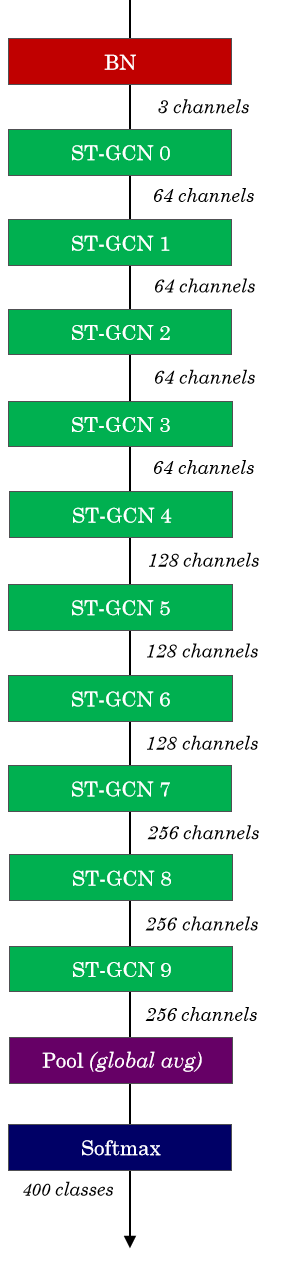
\includegraphics[width=3.2cm]{images/st_gcn_architecture}
    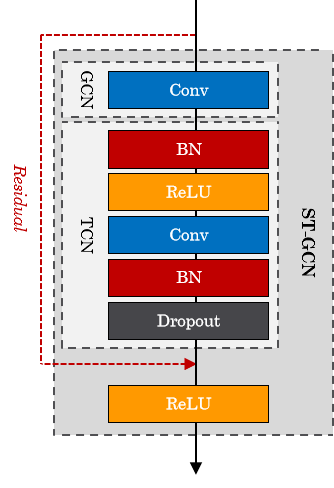
\includegraphics[width=3.5cm]{images/st_gcn_architeture_unit}
    \caption{Visão geral da arquitetura do modelo (à esquerda) e detalhe de uma unidade do ST-GCN (à direita).}
    \label{fig:st-gcn-architecture}
\end{figure}


\section{Dataset} %%%%%%%%%%%%%%%%%%%%%%%%%%%%%%%%%%%%%%%%%%%
\label{sec:dataset}
Será utilizado o \textit{dataset} \textit{American Sign Language Lexicon Video Dataset} (ASLLVD)\footnote{
    \textit{American Sign Language Lexicon Video Dataset} (ASLLVD) - disponível no endereço \url{http://vlm1.uta.edu/~athitsos/asl_lexicon/}
}, que é composto por vídeos de sinais realizados por diferentes atores, com diferentes níveis de fluência na língua de sinais. O \textit{dataset} também contém arquivos de metadados que determinam o nome e os respectivos \textit{frames} de início e fim para os sinais nos vídeos gravados. Ele é apresentado em mais detalhes em \cite{athitsos-asldataset-2008}.

\image
    {fig:asllvd-example}
    {images/asllvd_example}
    {Exemplo de representação do sinal \textit{"MERRY-GO-ROUND"} capturado em três perspectivas distintas no \textit{dataset} ASLLVD \cite{athitsos-asldataset-2008}.}

Para que os vídeos possam ser utilizados como entrada para o modelo ST-GCN, é necessário antes realizar um pré-processamento consistindo nas seguintes etapas:
\begin{enumerate}
    \item Segmentar vídeos: as amostras do  ASLLVD compreendem seções onde foram gravados vários sinais em sequência. Devido a isso, é necessário segmentá-los em vários vídeos contendo sinais individuais, utilizando para isso os arquivos de metadados disponibilizados com o \textit{dataset}, que indicam os momentos de início e término de cada sinal;
    \item Aumentar \textit{dataset}: foi observado no \textit{dataset} acima que não há um grande número de variações para os sinais contidos. Existe geralmente 1 ou 2 vídeos por sinal e, para melhorar o desempenho do modelo, será necessário gerar variações a partir dos vídeos existentes;
    \item Estimar pose: em seguida, é necessário extrair os pontos do corpo dos atores para cada frame dos vídeos, através da biblioteca OpenPose para em seguida agrupá-los em um único arquivo JSON. Para o propósito deste projeto serão considerados 130 pontos, ou seja, além dos 18 pontos referentes ao corpo estão inclusos também os 70 pontos da face e 21 pontos para cada uma das mãos, conforme ilustrado na \refimage{fig:keypoints-face-hand};
    \item Preencher frames vazios: todas as amostras utilizadas na entrada do modelo devem possuir tamanho uniforme, conforme descrito em \cite{st-gcn-2018}. Para isso, os autores sugerem que a sequência de frames dos vídeos seja repetida até completar o tamanho de entrada, que para este trabalho será de 10 segundos (ou 30es, considerando a taxa de 30 fps);
    \item Dividir grupos de amostras: separar as amostras pré-processadas entre os grupos treinamento e validação, com uma proporção de 80\% e 20\%, respectivamente;
    \item Serializar amostras: a implementação do ST-GCN utiliza como entradas listas de objetos do Python serializados e gravados como arquivos \textit{.pkl} em disco. Sendo assim, esse processo deve ser aplicado aos conjuntos de amostras divididos no passo anterior.
\end{enumerate}

\begin{figure}[ht]
    \centering
    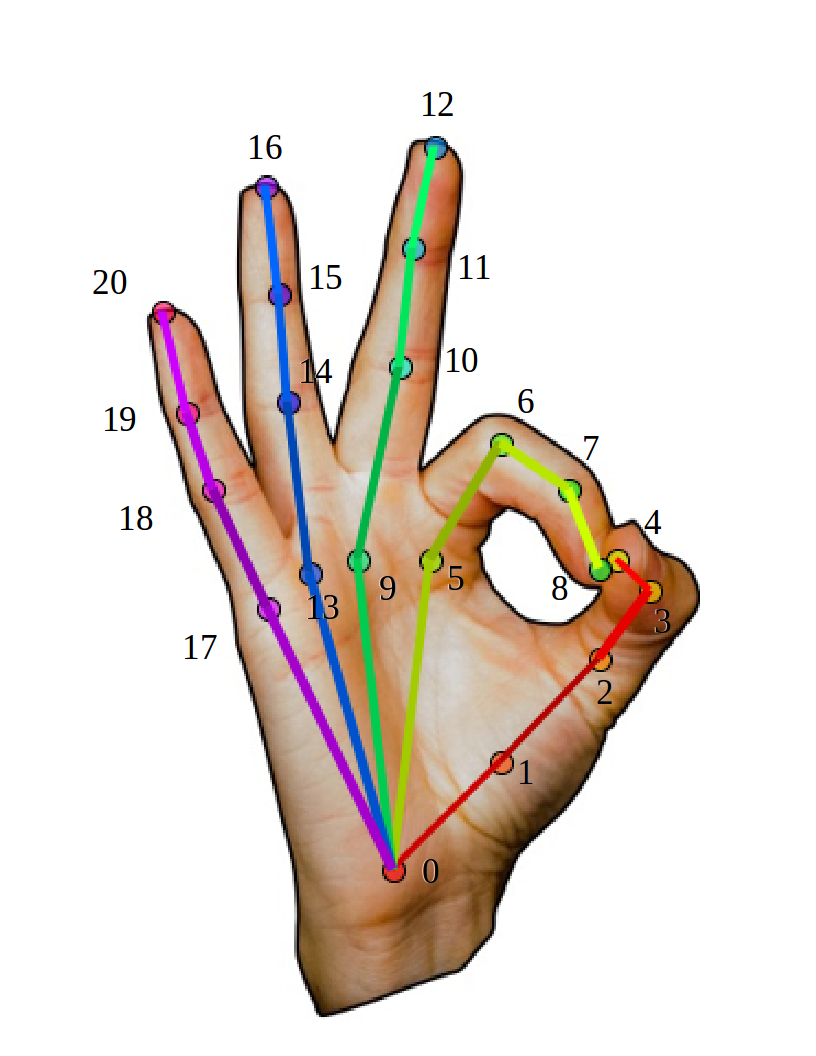
\includegraphics[width=3cm]{images/keypoints_hand}
    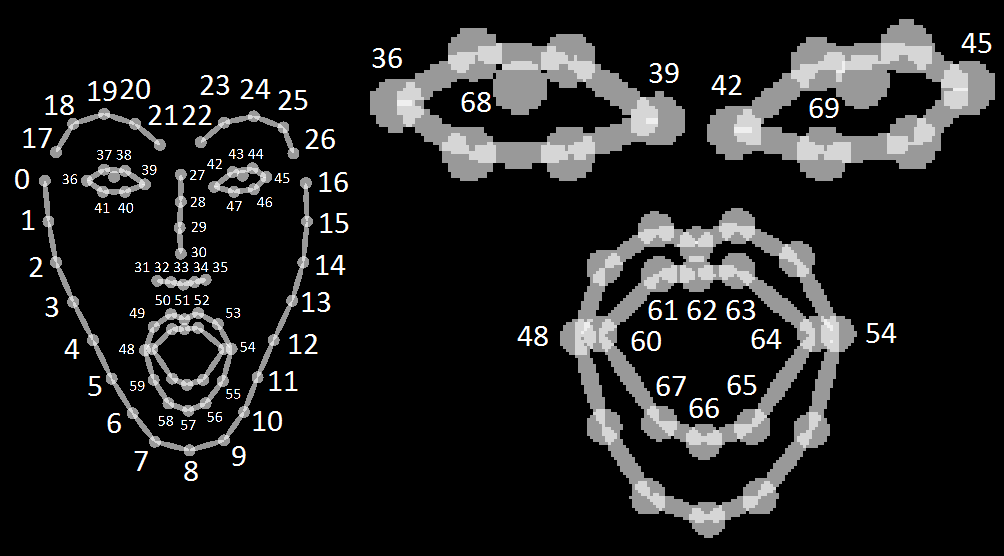
\includegraphics[width=5cm]{images/keypoints_face}
    \caption{Representação dos 21 pontos da mão e 70 pontos da face extraídos pelo OpenPose e que serão utilizados neste trabalho.}
    \label{fig:keypoints-face-hand}
\end{figure}
Como os sinais contidos no \textit{dataset} não possuem sua descrição em CORE-SL, será necessário produzir as respectivas \textit{labels} nesse formato. Entretanto, o tempo limitado para execução deste trabalho, atua como limitador na produção dessas \textit{labels} e quantidade de amostras classificadas dessa forma que será possível obter a tempo de aplicar ao modelo e extrair resultados. Uma das estratégias para lidar com isso é selecionar um conjunto de cerca das 20 características mais relevantes do CORE-SL para classificar os vídeos no primeiro momento. O CORE-SL possui um total de 100 características.


\section{Etapas da pesquisa} %%%%%%%%%%%%%%%%%%%%%%%%%%%%%%%%%%%%%%%%%%%
Com o intuito de lidar com os problemas apresentados acima, como a necessidade de criação do  \textit{dataset} em CORE-SL e a demanda por recursos computacionais elevados para execução dos algoritmos de estimação de pose e do ST-GCN, esta pesquisa foi segmentada em duas etapas. 

A primeira delas, consiste em atuar na adaptação das camadas de entrada e nas representações internas do modelo ST-GCN para fazê-lo considerar os grafos com os novos pontos do corpo e utilizar a nova base de dados para seu treinamento. Nesse momento, objetiva-se conhecer o desempenho do modelo frente ao problema da língua de sinais e, dessa forma, os sinais serão classificados segundo seu nome já contido na base ASLLVD (dispensando a necessidade do \textit{dataset} em CORE-SL). Em termos gerais, essa etapa engloba:
\begin{enumerate}
    \item Localizar \textit{dataset} de língua de sinais (concluído);
    \item Criar pipeline de pré-processamento do \textit{dataset} para o ST-GCN (concluído);
    \item Aumentar \textit{dataset} para adicionar variações aos vídeos;
    \item Adaptar ST-GCN e suas representações de grafos (em andamento);
    \item Treinar modelo adaptado (em andamento);
    \item Avaliar e melhorar resultados.
\end{enumerate}

Na segunda etapa, as camadas finais do modelo deverão ser adaptadas e a saída do modelo deverá estar no formato das características fonológicas criadas para o novo \textit{dataset} em CORE-SL. Aqui também será necessário definir uma estratégia para representação dessas características pelo classificador. Essa etapa considera os seguintes passos:
\begin{enumerate}
    \item Criar \textit{labels} em CORE-SL para o \textit{dataset};
    \item Definir estratégia para representação das saídas do ST-GCN como características fonológicas;
    \item Adaptar as camadas de saída do ST-GCN para considerar a estratégia acima;
    \item Treinar modelo adaptado;
    \item Avaliar e melhorar resultados.
\end{enumerate}

Atualmente, a maioria dos passos definidos para a primeira etapa encontram-se em andamento, seguindo um ciclo de adaptação, treinamento e correção/otimização.


% Bibliografia
\bibliographystyle{IEEEtran}
\bibliography{IEEEabrv,references.bib}

\end{document}
%%